\section{Marching cubes}
\label{sec:marching_cubes}
The geometry in DSMC is represented as voxels as we discussed in section \ref{sec:dsmc_complex_geometries}. They form a scalar field with values zero for empty voxels, and non-zero for filled voxels. The surface of the geometry is where the values of the scalar field \textit{changes} from zero to a non-zero value. This defines the \textit{isosurface}, i.e. a surface where all the values on one side is zero, and non-zero on the other side. If we find a way to visualize this isosurface, it will coincide with where the DSMC particles collide. We then need to create some primitives (in this case triangles) that are connected to each other forming a the full isosurface. Luckily for us, such an algorithm exists and is called \textit{marching cubes}.\\
Marching cubes is an algorithm used to generate a set of connected triangles from the isosurface of a scalar field. The method was presented in a paper published in 1987 and has been widely used in medical visualizations of CT and MRI scans\cite{wiki:marching_cubes}. Assuming that the scalar field is discretized in space, each point (vertex) either has a value larger than some chosen iso-value, or a smaller value. Given a cube consisting of eight of these vertices, there exists $2^{8}=256$ unique combinations (each vertex has two possibilities). Because of symmetries (a cube with only one vertex being larger than the iso-value has through rotations 8 different configurations that really are the same configuration), this set can be reduced to 15. In figure \ref{fig:vis_marching_cubes}, we see the 15 unique configurations and the corresponding triangles in each configuration.
\begin{figure}[h]
\begin{center}
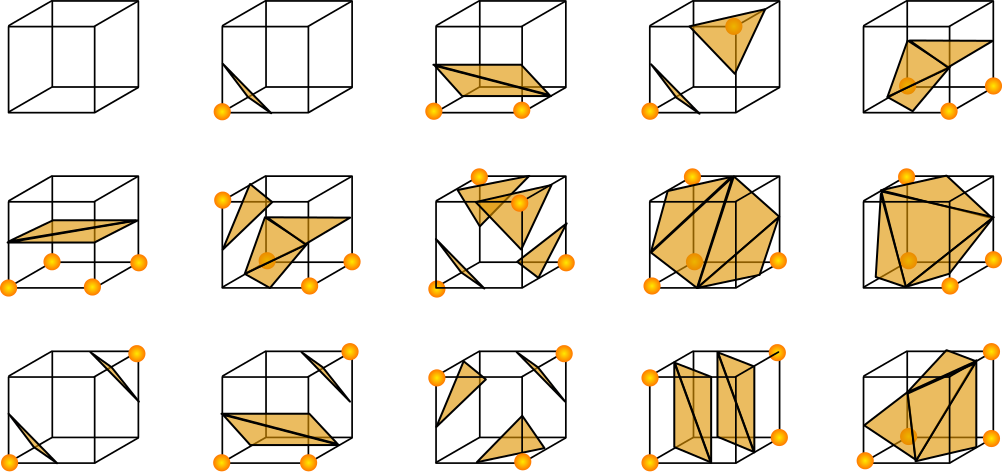
\includegraphics[width=\textwidth, trim=0cm 0cm 0cm 0cm, clip]{visualizations/figures/marching_cubes.png}
\end{center}
\caption{A cube consisting of eight vertices, each having a value smaller or larger than a given iso-value has $2^8=256$ different combinations. This number can due to symmetries be reduced to 15 as we see here. (Image from \url{http://en.wikipedia.org/wiki/File:MarchingCubes.svg}, accessed 20 March, 2014.)}
\label{fig:vis_marching_cubes}
\end{figure}
For a given cube, the 8 vertex values (one or zero) can be represented as the bits in an 8-bit integer. The final value of this integer is then the index of a pre-computed table containing a list of all triangles needed for that configuration. Well, the authors thought the 15 combinations would be enough, but it turns out that with these 15 configurations, there exists cases where the surface gets holes. This is topologically incorrect (the surface should not have any holes). This problem was solved in 1995 by using a larger set with 33 unique configurations which spans out the full configuration space \cite{chernyaev1995marching}.\\
Since the geometry in DSMC model is described by a scalar field with values zero, one and two, we can choose iso-value of one and use the marching cube algorithm to generate triangles we can render on the GPU. 